\definecolor{refining_pv}{RGB}{209,73,75}
\definecolor{ammonia_pv}{RGB}{252,186,29}
\definecolor{otherpure_pv}{RGB}{109,204,220}
\definecolor{methanol_pv}{RGB}{94,71,128}
\definecolor{dri_pv}{RGB}{168,149,196}
\definecolor{othermixed_pv}{RGB}{203,203,203}

\makeatletter
\newcommand\resetstackedplots{
\makeatletter
\pgfplots@stacked@isfirstplottrue
\makeatother
\addplot [forget plot,draw=none] coordinates{(2000,0) (2005,0) (2010,0) (2015,0) (2018,0)};
}
\makeatother

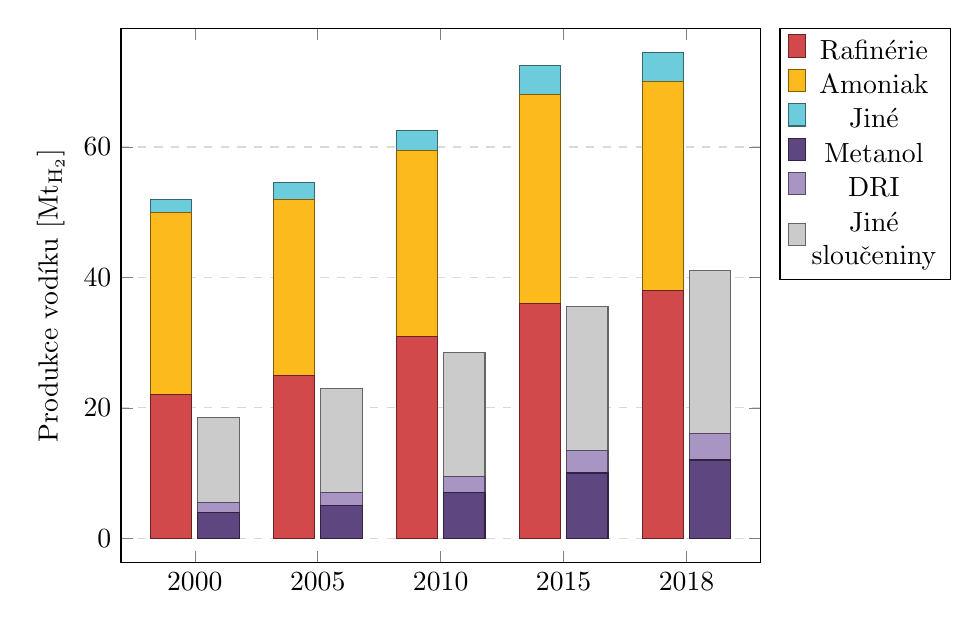
\begin{tikzpicture}
    \begin{axis}[
        ybar stacked,
        width = 0.8\textwidth,
        ymajorgrids,
        grid style={dashed,gray!30},
	bar width=15pt,
        enlarge x limits=0.15,
        enlarge y limits=0.05,
        ymin = 0,
        legend style={cells={align=center}},
        legend entries={Rafinérie,Amoniak,Jiné,Metanol,DRI,Jiné\\sloučeniny},
        legend pos=outer north east,
        ylabel={Produkce vodíku $[\mathrm{Mt_{H_2}}]$},
        symbolic x coords={2000,2005,2010,2015,2018},
        xtick=data,
    ]
        \addplot+[ybar,refining_pv!50!black,fill=refining_pv,text=black,bar shift=-.3cm] plot coordinates {(2000,22) (2005,25) (2010,31) (2015,36) (2018,38)};
        \addplot+[ybar,ammonia_pv!50!black,fill=ammonia_pv,text=black,bar shift=-.3cm] plot coordinates {(2000,28) (2005,27) (2010,28.5) (2015,32) (2018,32)};
        \addplot+[ybar,otherpure_pv!50!black,fill=otherpure_pv,text=black,bar shift=-.3cm] plot coordinates {(2000,2) (2005,2.5) (2010,3) (2015,4.5) (2018,4.5)};
        \resetstackedplots
        \addplot+[ybar,methanol_pv!50!black,fill=methanol_pv,text=black,bar shift=+.3cm] plot coordinates {(2000,4) (2005,5) (2010,7) (2015,10) (2018,12)};
        \addplot+[ybar,dri_pv!50!black,fill=dri_pv,text=black,bar shift=+.3cm] plot coordinates {(2000,1.5) (2005,2) (2010,2.5) (2015,3.5) (2018,4)};
        \addplot+[ybar,othermixed_pv!50!black,fill=othermixed_pv,text=black,bar shift=+.3cm] plot coordinates {(2000,13) (2005,16) (2010,19) (2015,22) (2018,25 )};
    \end{axis}
\end{tikzpicture}